

\tikzset{every picture/.style={line width=0.75pt}} %set default line width to 0.75pt        

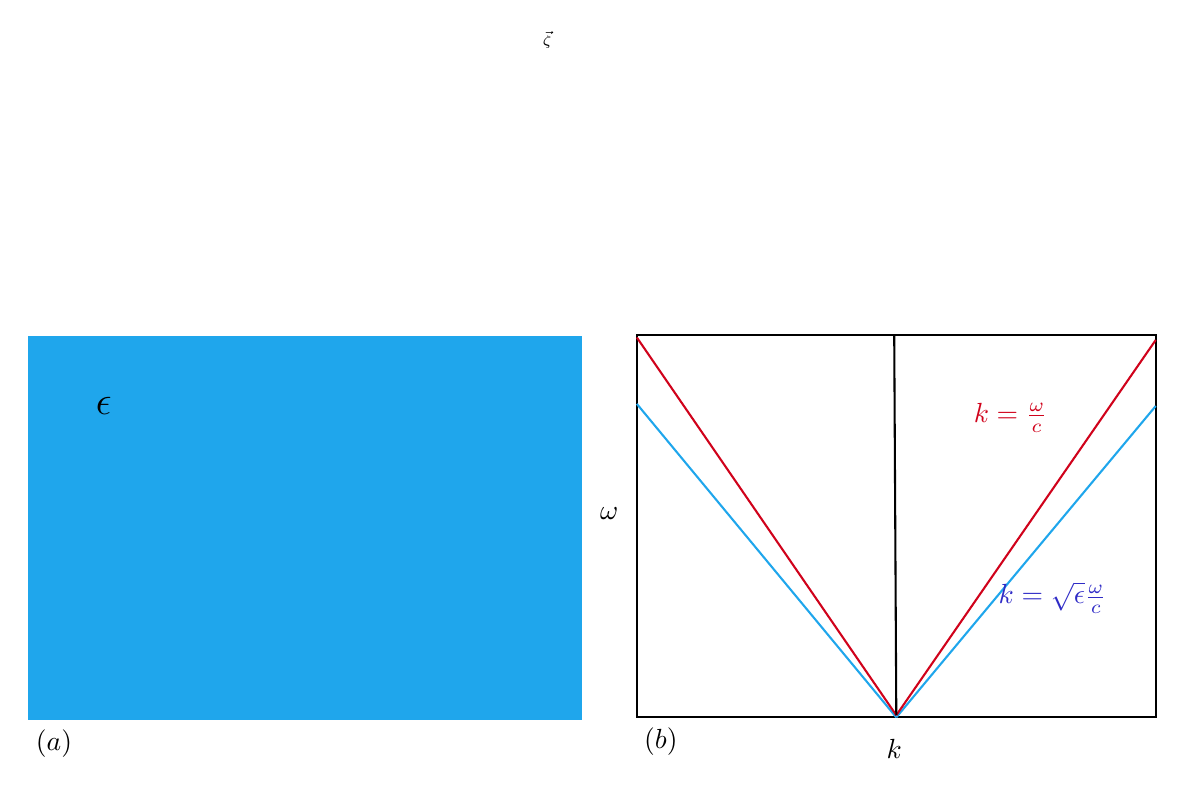
\begin{tikzpicture}[x=0.75pt,y=0.75pt,yscale=-1,xscale=1]
%uncomment if require: \path (0,300); %set diagram left start at 0, and has height of 300

%Shape: Rectangle [id:dp2370189011099142] 
\draw   (346.17,40) -- (596.17,40) -- (596.17,224.17) -- (346.17,224.17) -- cycle ;
%Straight Lines [id:da9477212198255883] 
\draw [color={rgb, 255:red, 31; green, 166; blue, 236 }  ,draw opacity=1 ]   (346.17,73.17) -- (471.17,224.17) ;
%Straight Lines [id:da38120967955829277] 
\draw [color={rgb, 255:red, 31; green, 166; blue, 236 }  ,draw opacity=1 ]   (596.17,74.17) -- (471.17,224.17) ;

%Straight Lines [id:da8438048623151154] 
\draw [color={rgb, 255:red, 208; green, 2; blue, 27 }  ,draw opacity=1 ]   (346.17,41.17) -- (471.17,223.17) ;
%Straight Lines [id:da6201464061225517] 
\draw [color={rgb, 255:red, 208; green, 2; blue, 27 }  ,draw opacity=1 ]   (596.17,42.37) -- (471.17,223.17) ;

%Straight Lines [id:da8440907794928258] 
\draw    (471.17,223.17) -- (470.17,40.17) ;

%Shape: Rectangle [id:dp06864759116466967] 
\draw  [color={rgb, 255:red, 31; green, 166; blue, 236 }  ,draw opacity=1 ][fill={rgb, 255:red, 31; green, 166; blue, 236 }  ,fill opacity=1 ] (53.17,41) -- (319.17,41) -- (319.17,225.17) -- (53.17,225.17) -- cycle ;



% Text Node
\draw (299,-107.6) node [anchor=north west][inner sep=0.75pt]  [font=\tiny]  {$\vec{\mathbf{\zeta }}$};
% Text Node
\draw (55.17,228.57) node [anchor=north west][inner sep=0.75pt]    {$( a)$};
% Text Node
\draw (84,68.4) node [anchor=north west][inner sep=0.75pt]  [font=\Large]  {$\epsilon $};
% Text Node
\draw (348.17,227.57) node [anchor=north west][inner sep=0.75pt]    {$( b)$};
% Text Node
\draw (519,157.4) node [anchor=north west][inner sep=0.75pt]  [color={rgb, 255:red, 47; green, 43; blue, 198 }  ,opacity=1 ]  {$k=\sqrt{\epsilon }\frac{\omega }{c}$};
% Text Node
\draw (507,71.4) node [anchor=north west][inner sep=0.75pt]  [color={rgb, 255:red, 208; green, 2; blue, 27 }  ,opacity=1 ]  {$k=\frac{\omega }{c}$};
% Text Node
\draw (465,233.4) node [anchor=north west][inner sep=0.75pt]  [color={rgb, 255:red, 0; green, 0; blue, 0 }  ,opacity=1 ]  {$k$};
% Text Node
\draw (327,121.4) node [anchor=north west][inner sep=0.75pt]    {$\omega $};


\end{tikzpicture}
